\documentclass{article}
\usepackage[pdftex]{graphicx}
\usepackage{amsmath}
\usepackage{verbatim}
\usepackage{enumerate}
\author{Michael Anderson}
\title{Homework 5}
\begin{document}
\maketitle
\center{CS517}
\center{Prof. Cull}\\
\flushleft
\newpage

\section{}
Code is attached.

\section{}
Here are a couple of examples. When a random variable from the alphabet is
required, my implementation of the algorithm simply uses the first variable from
the first clause (sans any NOT symbol which might present there), making it
easy to see what the input to the next recursive call should look like.

\begin{verbatim}
andermic@mike-laptop:~/Desktop/cs517/hw5$ ./davis_putnam.py
Recursion 0: [['a', 'c', 'b'], ['c', 'b', 'a'], ['~a', 'b', 'c'], 
['~a', 'a', '~c'], ['a', 'b', '~b'], ['b', '~b', 'a']]
Recursion 1: [['b', 'c']]
Recursion 2: []
True

andermic@mike-laptop:~/Desktop/cs517/hw5$ ./davis_putnam.py
Recursion 0: [['~a', 'b', 'd'], ['~b', 'c', 'd'], ['a', '~c', 'd'],
['a', '~b', '~d'], ['b', '~c', '~d'], ['~a', 'c', '~d'], ['a', 'b', 'c'],
['~a', '~b', '~c']]
Recursion 1: [['b', 'd'], ['~b', 'c', 'd'], ['b', '~c', '~d'], 
['c', '~d'], ['~b', '~c']]
Recursion 2: [['c', 'd'], ['c', '~d'], ['~c']]
Recursion 3: [['d'], ['~d']]
Recursion 4: [[]]
Recursion 2: [['d'], ['~c', '~d'], ['c', '~d']]
Recursion 3: [['~c'], ['c']]
Recursion 4: [[]]
Recursion 1: [['~b', 'c', 'd'], ['~c', 'd'], ['~b', '~d'], 
['b', '~c', '~d'], ['b', 'c']]
Recursion 2: [['c', 'd'], ['~c', 'd'], ['~d']]
Recursion 3: [['c'], ['~c']]
Recursion 4: [[]]
Recursion 2: [['~c', 'd'], ['~c', '~d'], ['c']]
Recursion 3: [['d'], ['~d']]
Recursion 4: [[]]
False
\end{verbatim}

\section{}

\section{}
Code is attached.

\section{}
Following are graphs of probability of satisfiability as a function of density,
over various values of $n$ as indicated in the title of each graph. Most of the
data points are based on 100 samples at some particular density for some
particular $n$, a few of the computationally expensive points are based on 10
samples.

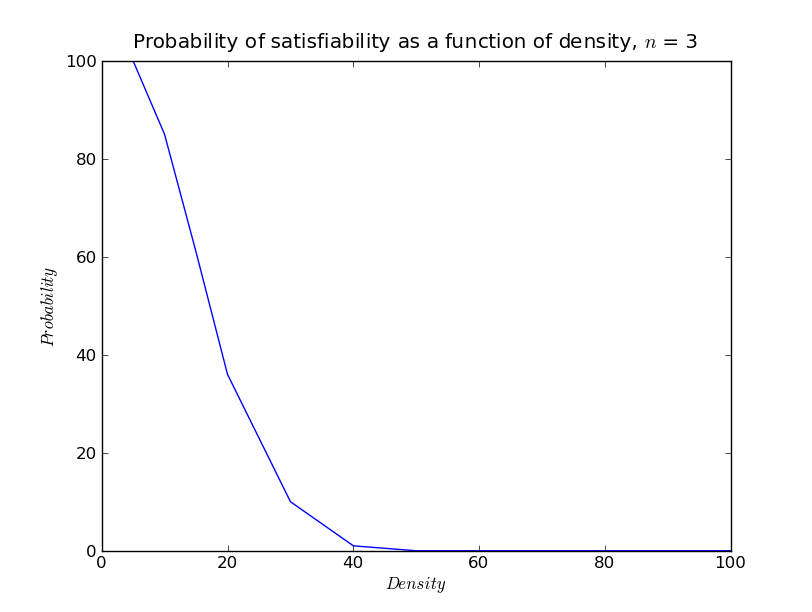
\includegraphics[scale=0.5]{probn3.png}
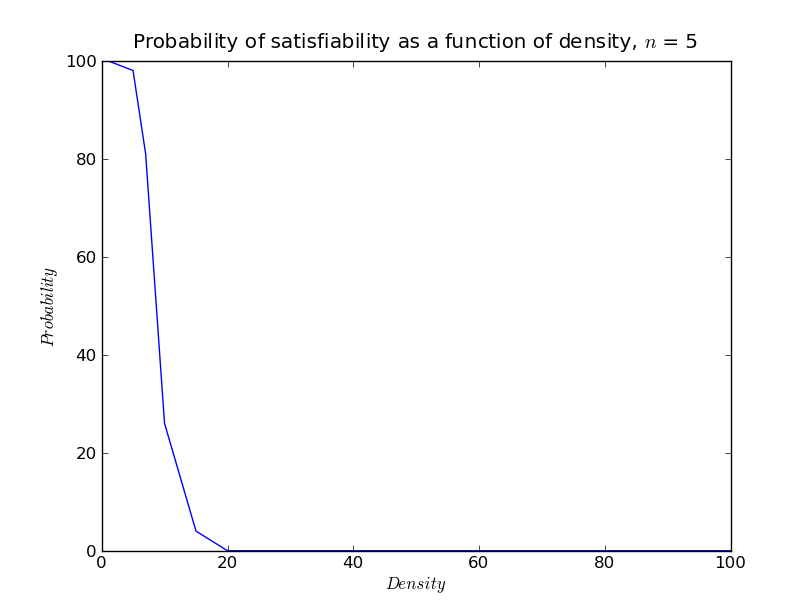
\includegraphics[scale=0.5]{probn5.png}
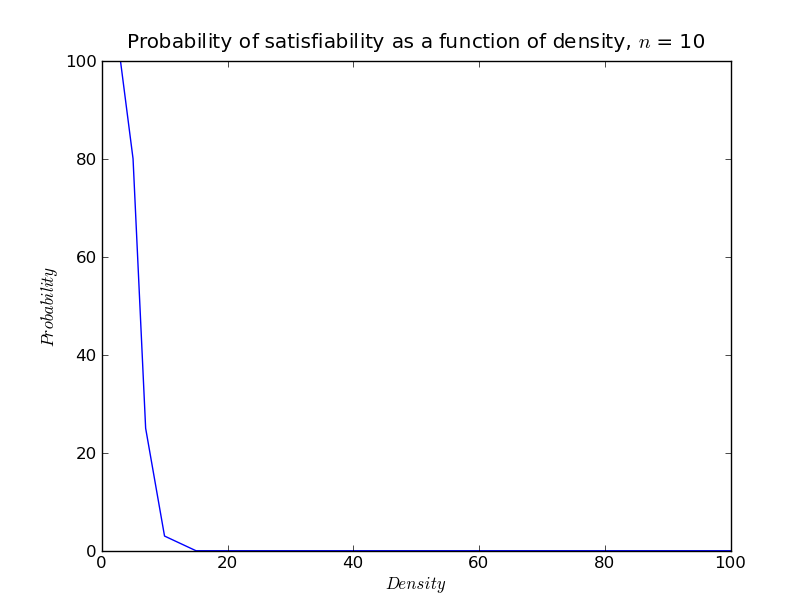
\includegraphics[scale=0.5]{probn10.png}
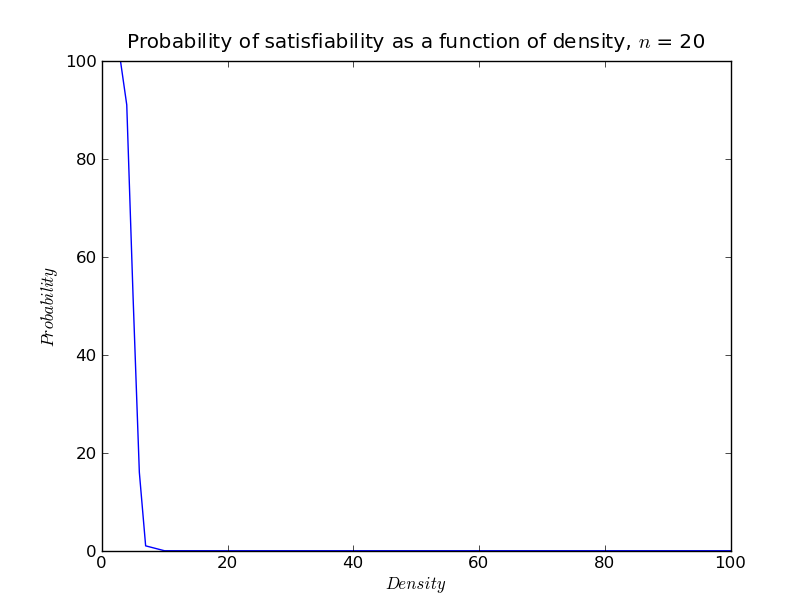
\includegraphics[scale=0.5]{probn20.png}
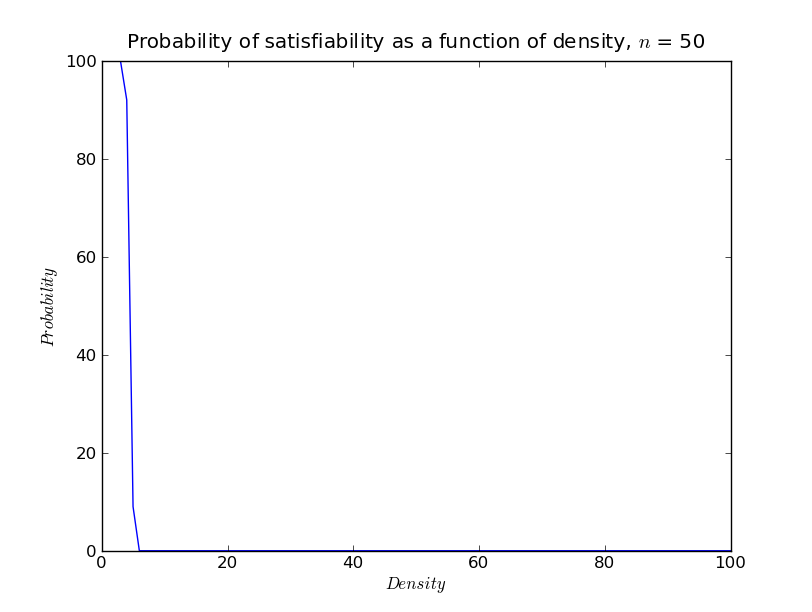
\includegraphics[scale=0.5]{probn50.png}
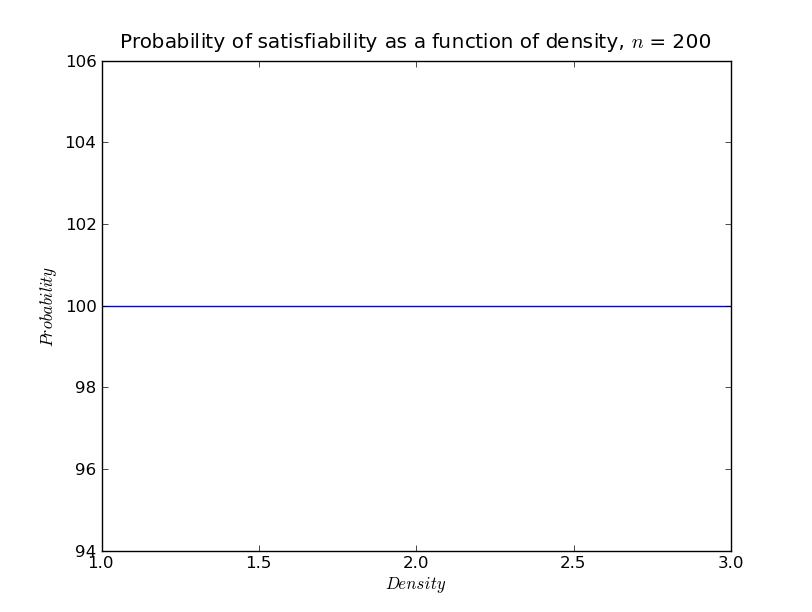
\includegraphics[scale=0.5]{probn200.png}
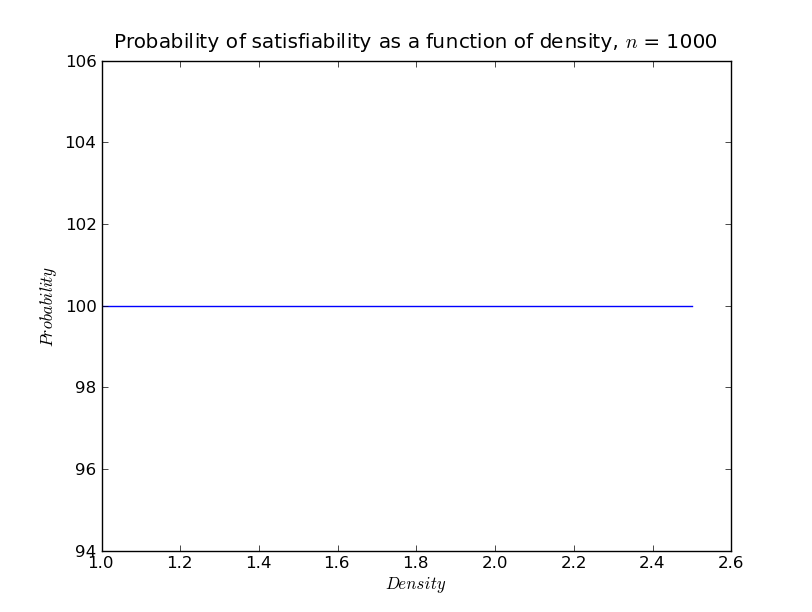
\includegraphics[scale=0.5]{probn1000.png}

So as expected, the probability of satisfiability decreases as a function of
density no matter the value of $n$. As $n$ gets large, it decreases faster.
For every value of $N$, for density $\le 3$, all of the generated boolean
functions were satisfiable.

\section{}
Following are average runtime of DP as a function of density for all of the
boolean functions generated and tested in (5). Number of samples for each data
point again range from 10 to 100.

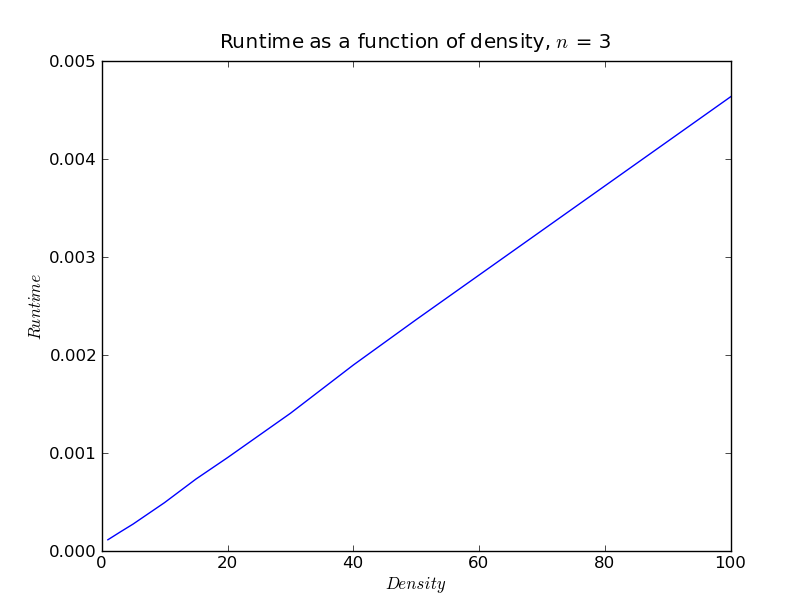
\includegraphics[scale=0.5]{timen3.png}
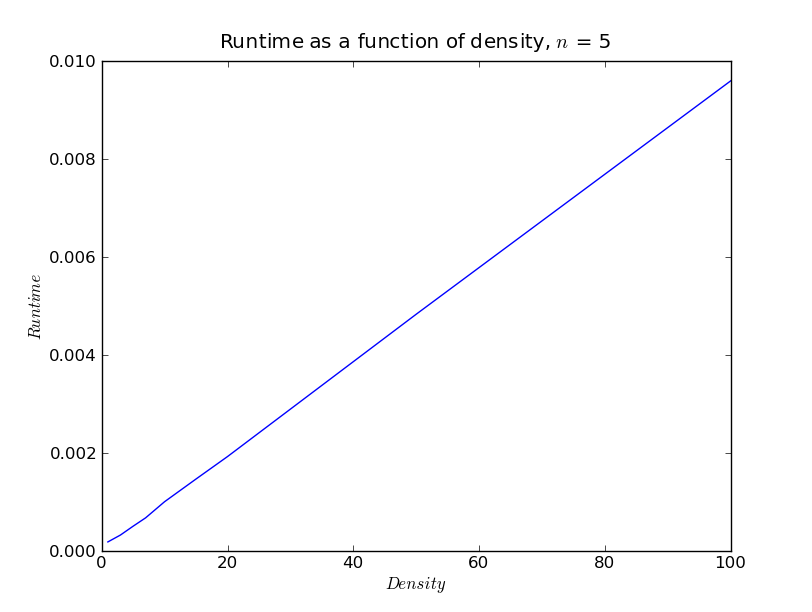
\includegraphics[scale=0.5]{timen5.png}
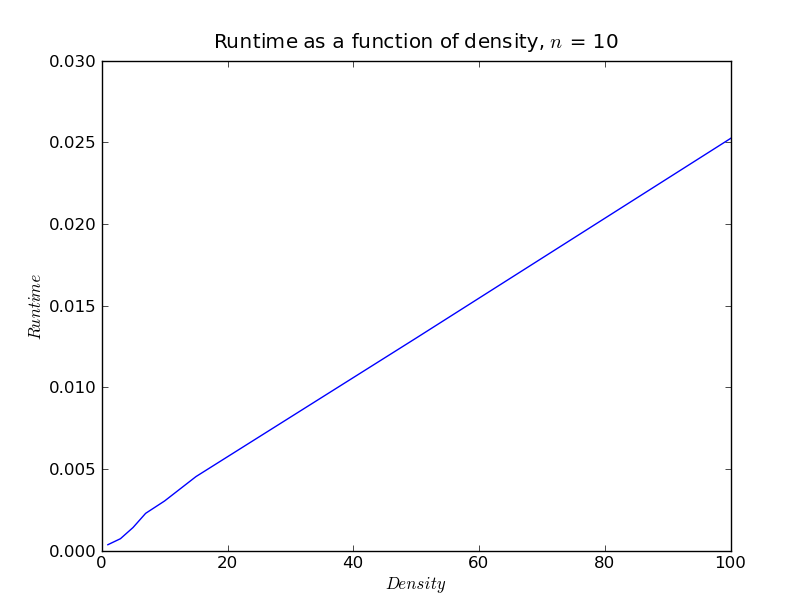
\includegraphics[scale=0.5]{timen10.png}
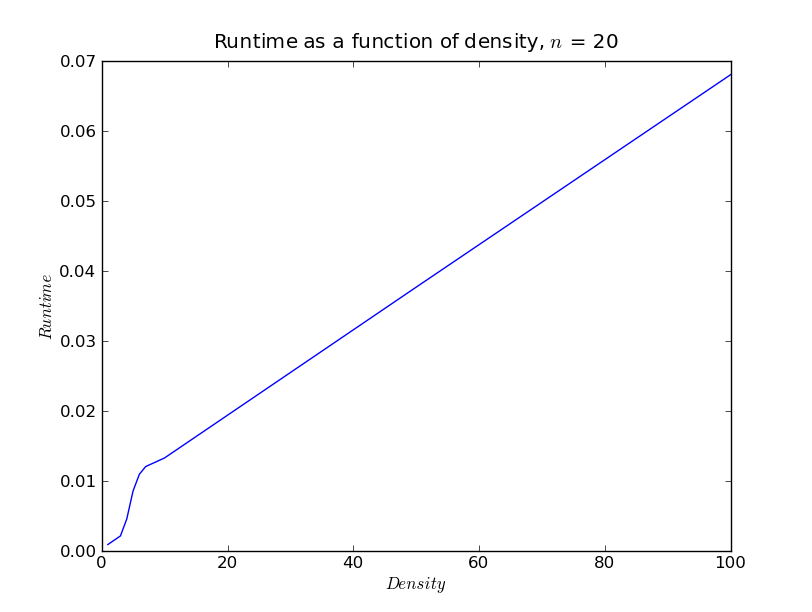
\includegraphics[scale=0.5]{timen20.png}
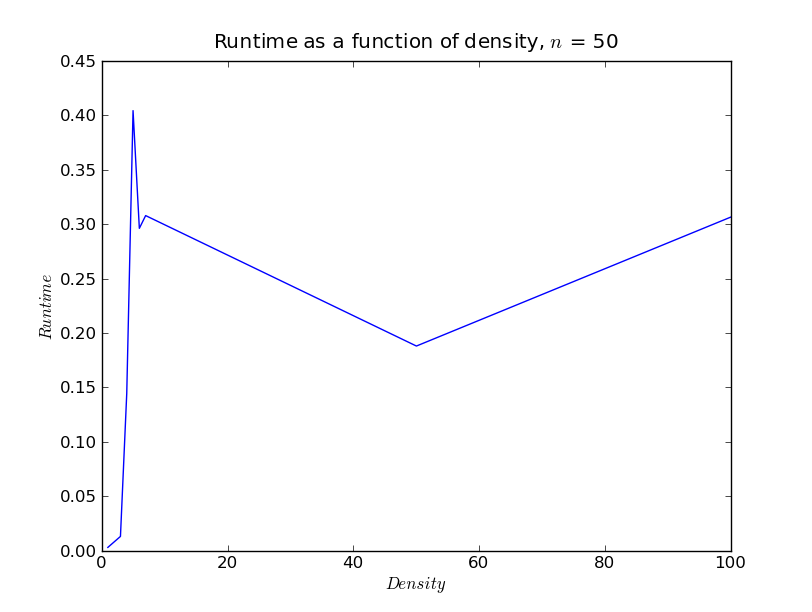
\includegraphics[scale=0.5]{timen50.png}
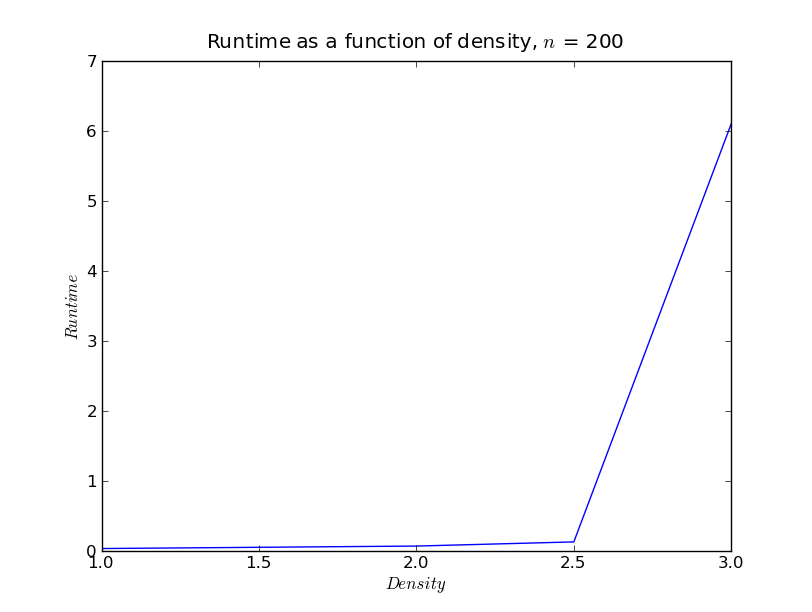
\includegraphics[scale=0.5]{timen200.png}
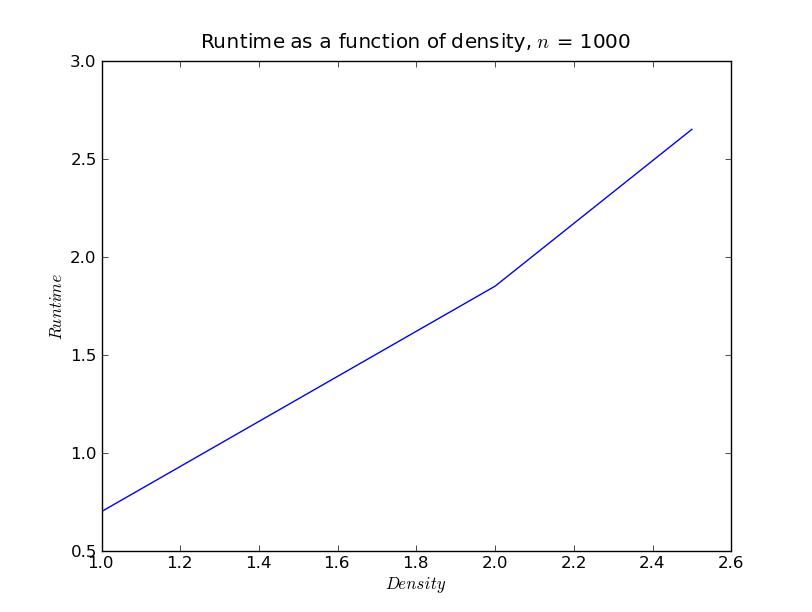
\includegraphics[scale=0.5]{timen1000.png}

Generally speaking, runtime seems to increase linearly as a function of both
density and $n$, for smaller values of $n$. As $n$ gets near and into the
triple digit range, the graphs show that runtime skyrockets as both $n$
increases and density increases.

\end{document}
